% =============================================================================
% RESULTS
% Status: DRAFT - Initial results documented
% =============================================================================

\subsection{Combined Spatial and Visual Analysis}

Figure~\ref{fig:combined} presents an integrated view of the Santa Ines drone survey analysis, demonstrating the fundamental difference between physical GPS locations and visual semantic clustering.

\begin{figure}[H]
    \centering
    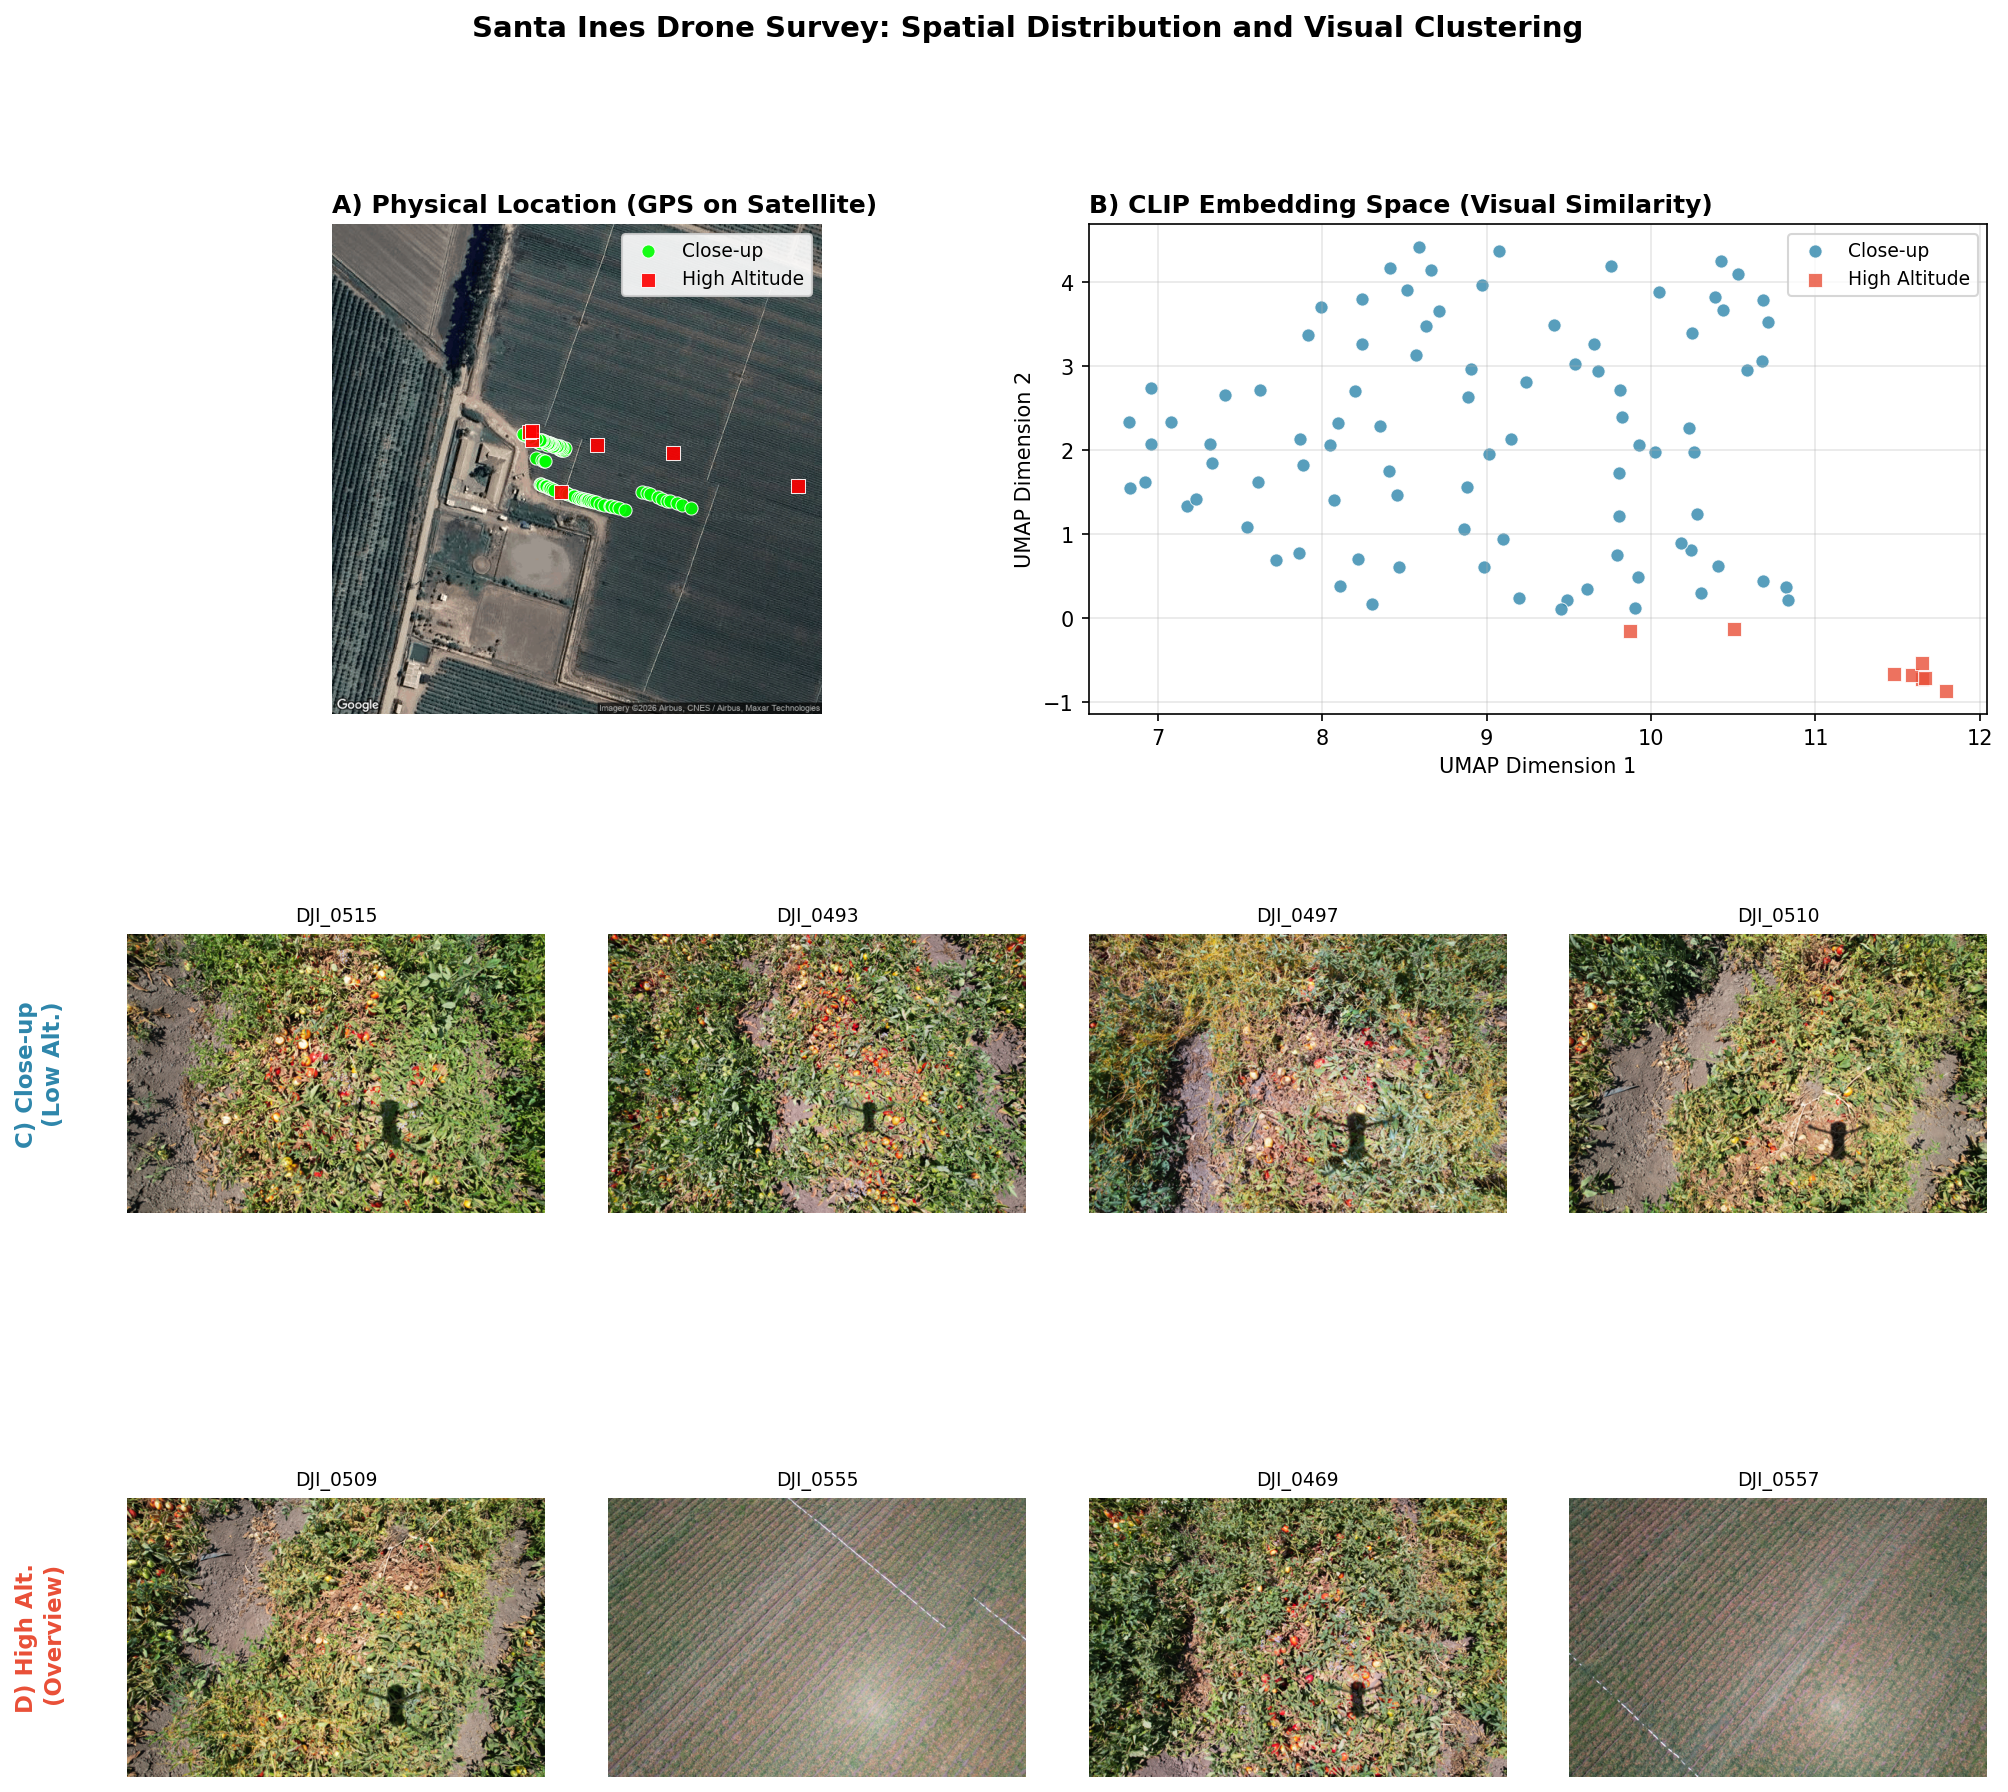
\includegraphics[width=\textwidth]{combined_analysis.png}
    \caption{Combined analysis of Santa Ines drone imagery. \textbf{(A)} GPS coordinates overlaid on satellite imagery showing flight coverage; \textbf{(B)} UMAP projection of CLIP embeddings revealing two semantic clusters; \textbf{(C)} Representative close-up images capturing detailed crop inspection views; \textbf{(D)} Representative high-altitude overview images showing vineyard row patterns.}
    \label{fig:combined}
\end{figure}

\subsubsection{GPS vs Visual Embedding: Key Differences}

Panel A reveals the physical flight pattern over the Santa Ines vineyard. The drone followed systematic transects across the crop rows, with close-up images (green markers) distributed along parallel flight lines and high-altitude overview images (red markers) captured at strategic positions across the field. Geographically, both image types are \textbf{spatially intermixed}---high-altitude shots were taken from various positions throughout the survey area.

In contrast, Panel B shows the CLIP embedding space where images cluster by \textbf{visual content rather than geographic location}. Despite being captured from scattered GPS positions, all high-altitude images form a tight cluster in the lower-right corner of the embedding space, clearly separated from the close-up images. This demonstrates that vision-language models organize images by semantic similarity (what the image depicts) rather than spatial proximity (where it was captured).

\subsubsection{Visual Characteristics of Each Cluster}

Panels C and D provide visual evidence for why CLIP separates these image categories:

\textbf{Close-up images (Panel C)} are characterized by:
\begin{itemize}
    \item High detail of individual vine plants and foliage
    \item Visible leaf texture, color variations, and plant structure
    \item Limited field-of-view showing 1-3 plant rows
    \item Rich color palette dominated by greens and earth tones
\end{itemize}

\textbf{High-altitude images (Panel D)} exhibit distinct visual patterns:
\begin{itemize}
    \item Geometric vineyard row patterns visible from above
    \item Uniform texture showing repetitive agricultural structure
    \item Wide field-of-view capturing dozens of rows
    \item Reduced color variation with dominant green/brown striping
\end{itemize}

\finding{CLIP embeddings successfully capture the semantic distinction between ``detailed crop inspection'' and ``field overview'' image types, enabling automatic categorization based purely on visual content}

\observation{This spatial-semantic decoupling has practical implications: images can be organized by content type regardless of capture location, enabling more intuitive dataset browsing and quality control workflows}

\subsection{Embedding Space Visualization}

CLIP embeddings projected to 2D via UMAP revealed two distinct clusters in the Santa Ines drone dataset (Figure~\ref{fig:embeddings}).

\begin{figure}[H]
    \centering
    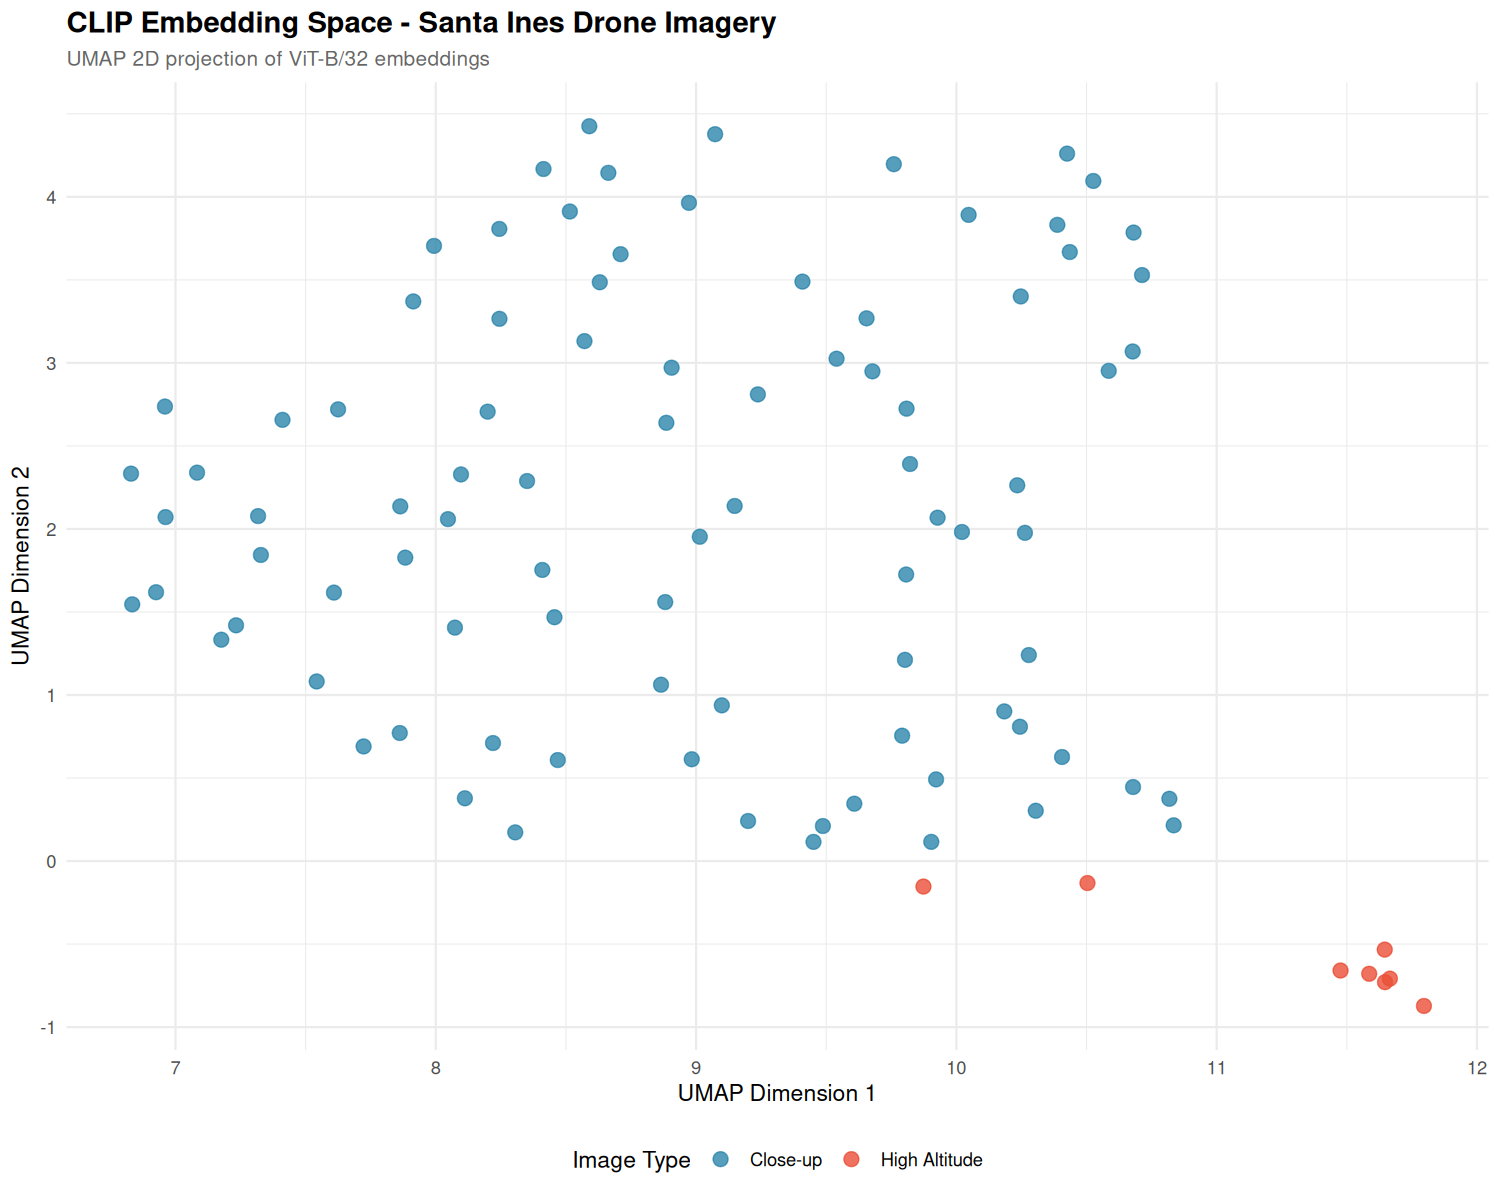
\includegraphics[width=0.9\textwidth]{r_embeddings_plot.png}
    \caption{UMAP projection of CLIP embeddings for 97 drone images. Blue points represent close-up crop inspection images; red points represent high-altitude overview images.}
    \label{fig:embeddings}
\end{figure}

\subsubsection{Cluster Characteristics}

\begin{table}[H]
\centering
\caption{Summary statistics for identified image clusters}
\label{tab:clusters}
\begin{tabular}{lcccc}
\toprule
\textbf{Category} & \textbf{Count} & \textbf{Percentage} & \textbf{UMAP X (mean $\pm$ sd)} & \textbf{UMAP Y (mean $\pm$ sd)} \\
\midrule
Close-up (crop inspection) & 89 & 91.8\% & $8.97 \pm 1.15$ & $2.15 \pm 1.28$ \\
High-altitude (overview) & 8 & 8.2\% & $11.30 \pm 0.70$ & $-0.56 \pm 0.27$ \\
\bottomrule
\end{tabular}
\end{table}

\observation{The high-altitude cluster shows lower variance (tighter grouping), suggesting more homogeneous visual content among overview images}

\subsubsection{Inter-cluster Distance}

The Euclidean distance between cluster centroids in UMAP space was \textbf{3.56 units}, indicating clear separation between semantic categories.

\subsection{Similarity Network Structure}

Network analysis of the 3-nearest-neighbor graph revealed strong within-cluster connectivity (Figure~\ref{fig:network}).

\begin{figure}[H]
    \centering
    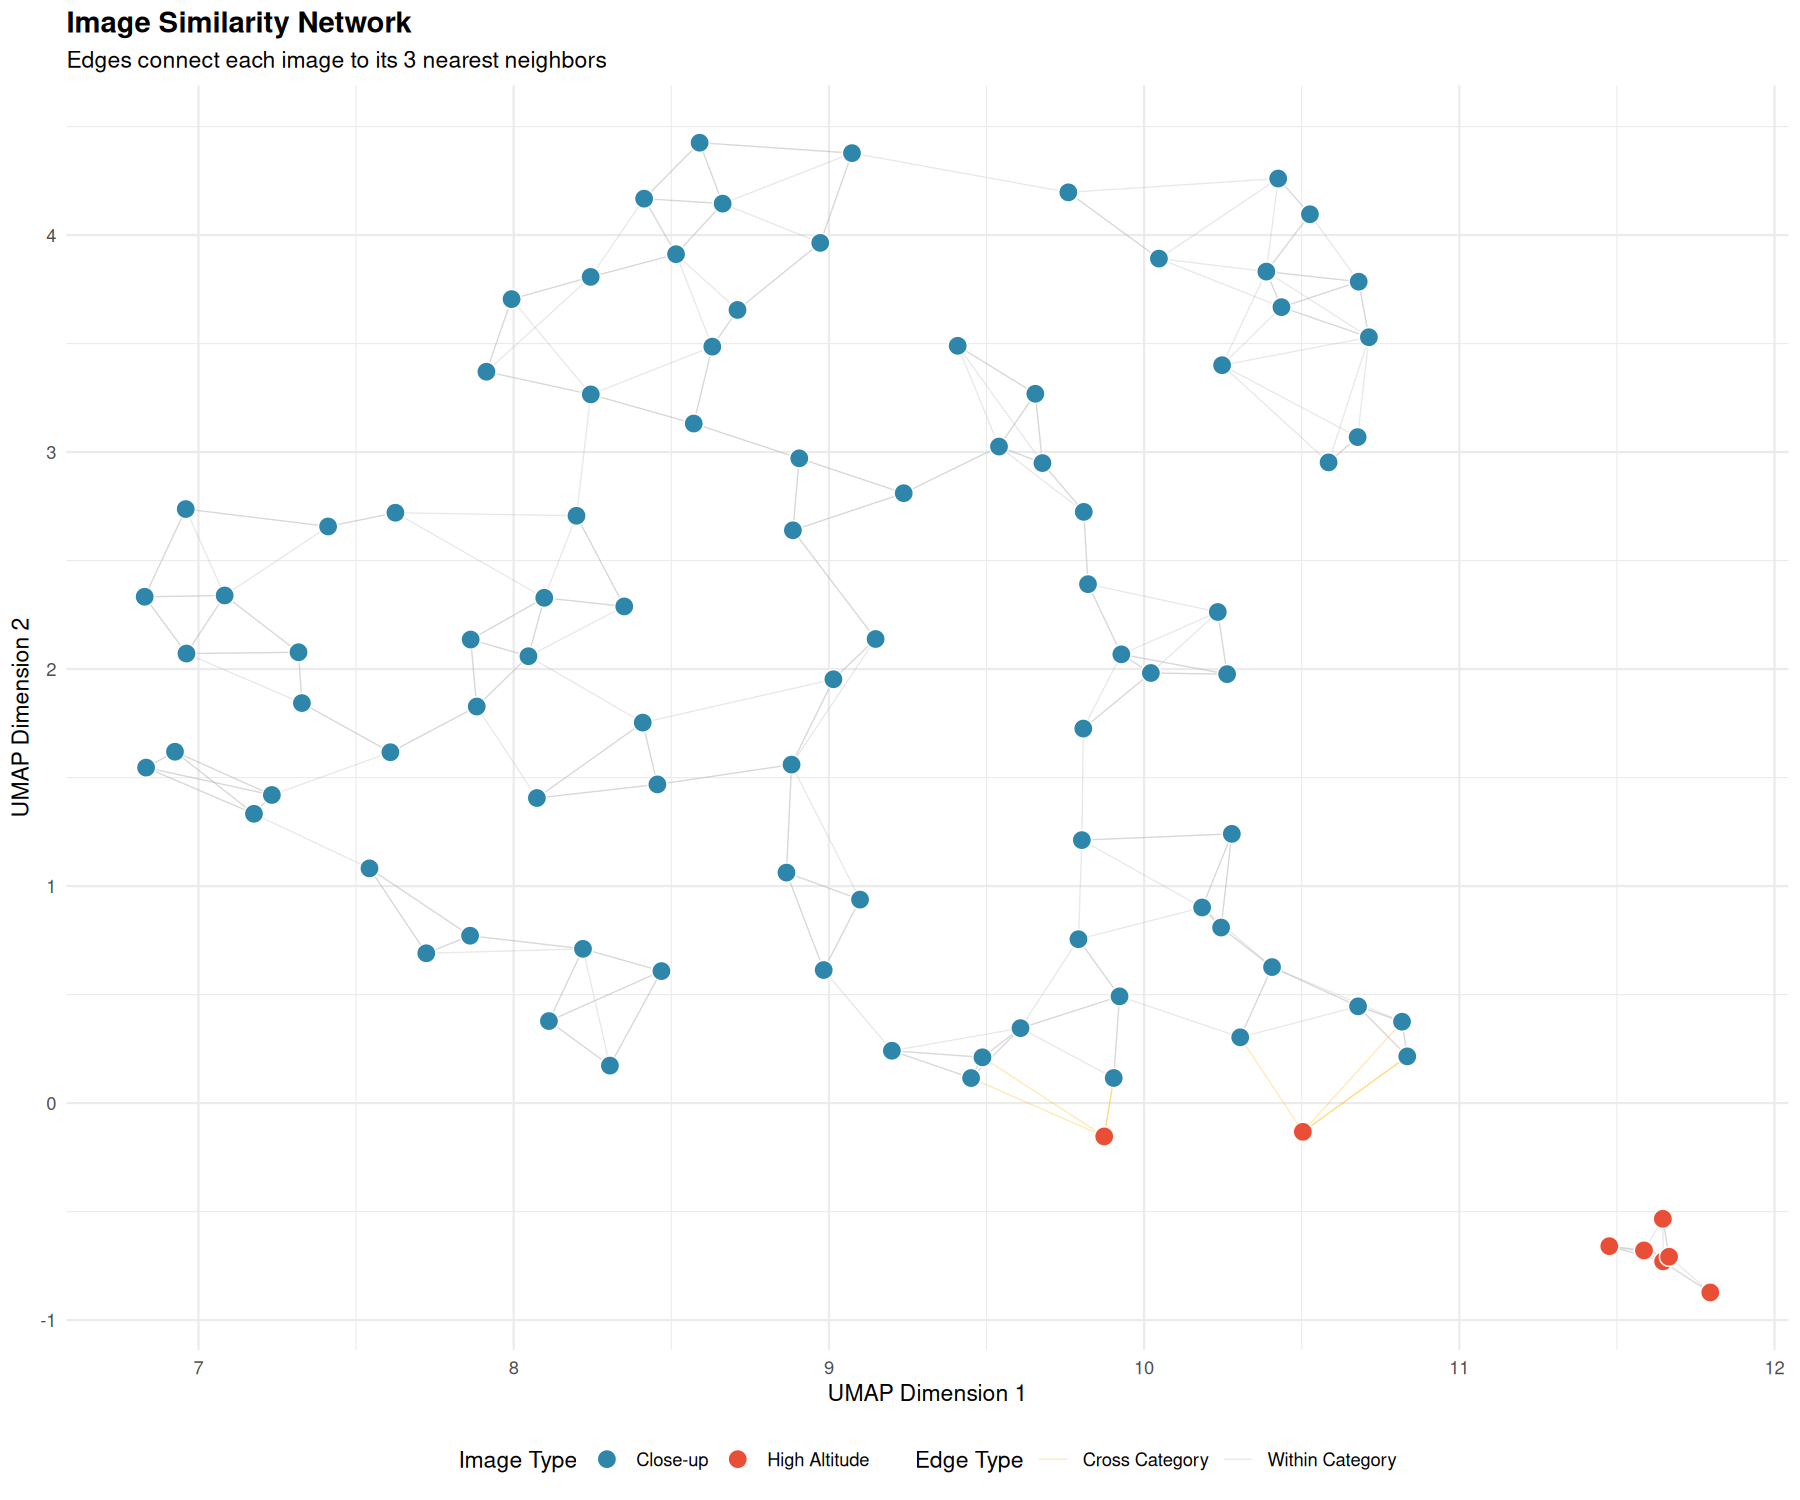
\includegraphics[width=0.95\textwidth]{r_similarity_network.png}
    \caption{Image similarity network. Nodes represent images (blue = close-up, red = high-altitude). Gray edges connect images within the same category; yellow edges indicate cross-category connections.}
    \label{fig:network}
\end{figure}

\subsubsection{Network Statistics}

\begin{itemize}
    \item \textbf{Total edges}: 291 (3 per image $\times$ 97 images)
    \item \textbf{Within-category edges}: 283 (97.3\%)
    \item \textbf{Cross-category edges}: 8 (2.7\%)
\end{itemize}

\finding{Only 2.7\% of nearest-neighbor connections cross category boundaries, confirming robust cluster separation}

\subsection{Cluster Cohesion Analysis}

Mean distance to 5 nearest neighbors was computed for each category (Figure~\ref{fig:cohesion}).

\begin{figure}[H]
    \centering
    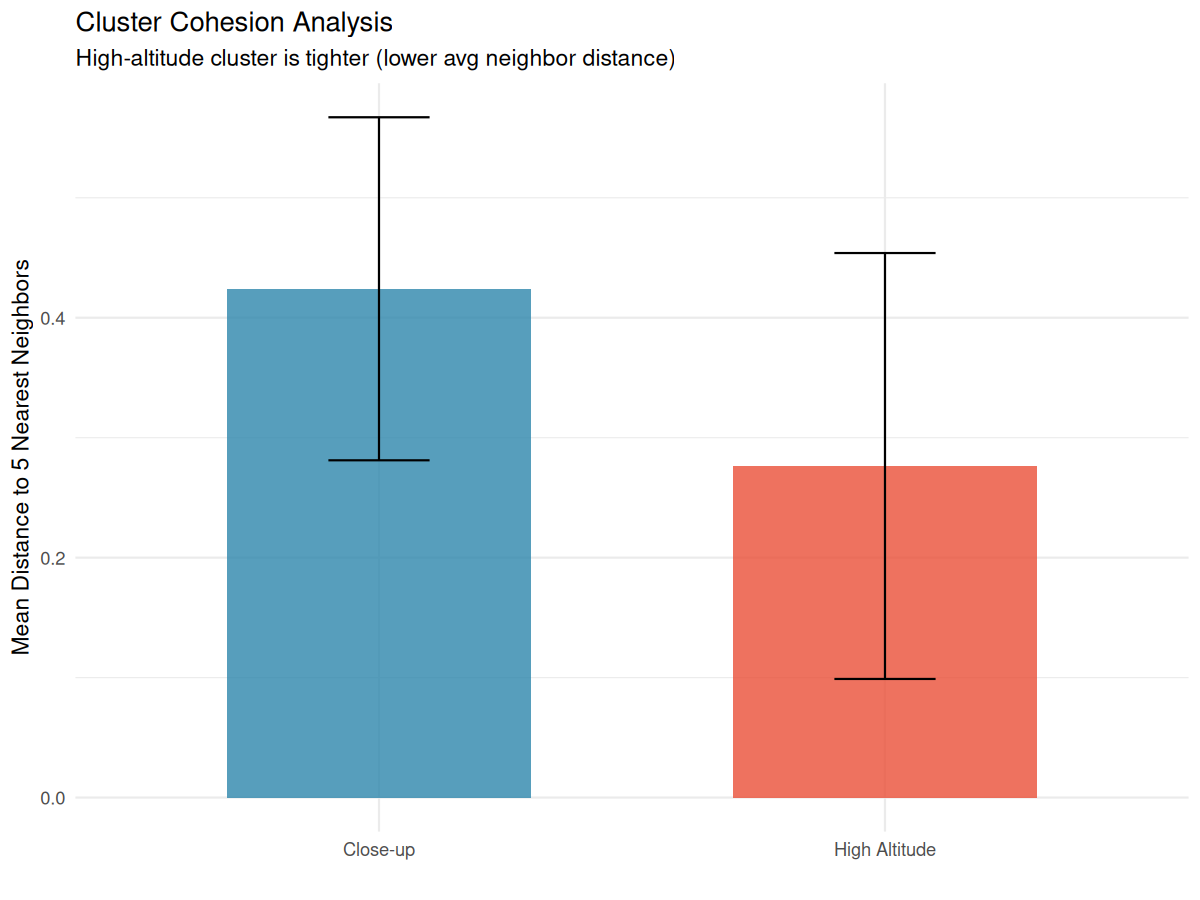
\includegraphics[width=0.7\textwidth]{r_cluster_cohesion.png}
    \caption{Cluster cohesion measured by mean distance to 5 nearest neighbors. Error bars show standard deviation.}
    \label{fig:cohesion}
\end{figure}

\begin{table}[H]
\centering
\caption{Cluster cohesion statistics}
\label{tab:cohesion}
\begin{tabular}{lccc}
\toprule
\textbf{Category} & \textbf{Mean Distance} & \textbf{Std Dev} & \textbf{n (neighbor pairs)} \\
\midrule
Close-up & 0.424 & 0.143 & 445 \\
High-altitude & 0.276 & 0.178 & 40 \\
\bottomrule
\end{tabular}
\end{table}

\observation{High-altitude cluster is 35\% more cohesive (lower neighbor distance) than the close-up cluster, despite having fewer samples}

\subsection{Image Size Analysis}

File size distribution showed modest differences between categories (Figure~\ref{fig:size}).

\begin{figure}[H]
    \centering
    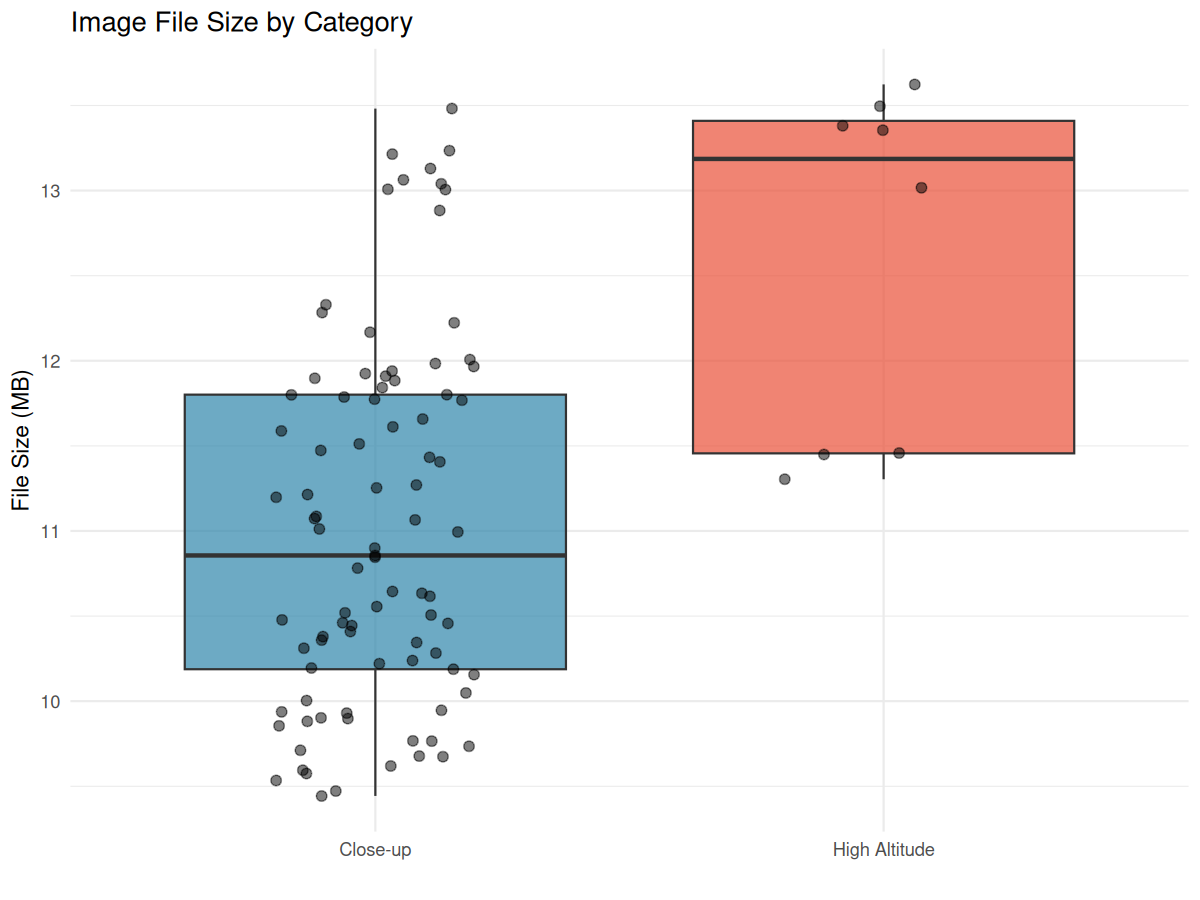
\includegraphics[width=0.7\textwidth]{r_size_analysis.png}
    \caption{Distribution of image file sizes by category.}
    \label{fig:size}
\end{figure}

\begin{itemize}
    \item Close-up images: mean 11.0 MB
    \item High-altitude images: mean 12.6 MB
\end{itemize}

\subsection{Similarity Search Validation}

Content-based image retrieval was tested using high-altitude images as queries. Results confirm that similarity search returns semantically consistent results:

\begin{table}[H]
\centering
\caption{Top-5 similar images for query DJI\_0552.JPG (high-altitude)}
\label{tab:similarity}
\begin{tabular}{clc}
\toprule
\textbf{Rank} & \textbf{Image} & \textbf{Category} \\
\midrule
1 & DJI\_0552.JPG & High-altitude (query) \\
2 & DJI\_0557.JPG & High-altitude \\
3 & DJI\_0555.JPG & High-altitude \\
4 & DJI\_0556.JPG & High-altitude \\
5 & DJI\_0554.JPG & High-altitude \\
\bottomrule
\end{tabular}
\end{table}

\finding{All top-5 results for a high-altitude query are also high-altitude images, demonstrating effective semantic retrieval}
